\section{Electrical Characterisation of Silicon Sensors}
\label{sec:setup}
The experimental setup and the procedure for the electrical characterisation of silicon sensors is presented in this section.
Although those tests were conducted at different locations, the following description is limited to the particular setup at CERN from which most of the results of this work were obtained.

\subsection{Setup at CERN}
\label{subsec:setup_alps}
At CERN, the S200FA probe station produced by Wentworth Laboratories Ltd. was in use for the electrical characterisation of neutron-irradiated silicon sensors. 
It is referred to as "Automatic-Low-Temperature Probe Station" (ALPS) because of its temperature-controlled chuck (produced by Systems att, C200-40 model) that can reach temperatures down to \SI{-40}{\celsius} and its programmable movements.
Apart from the power supply and meters, all relevant components were installed inside ALPS, see \ref{fig:ALPS_setup}.
\begin{figure}[h]
	\centering
	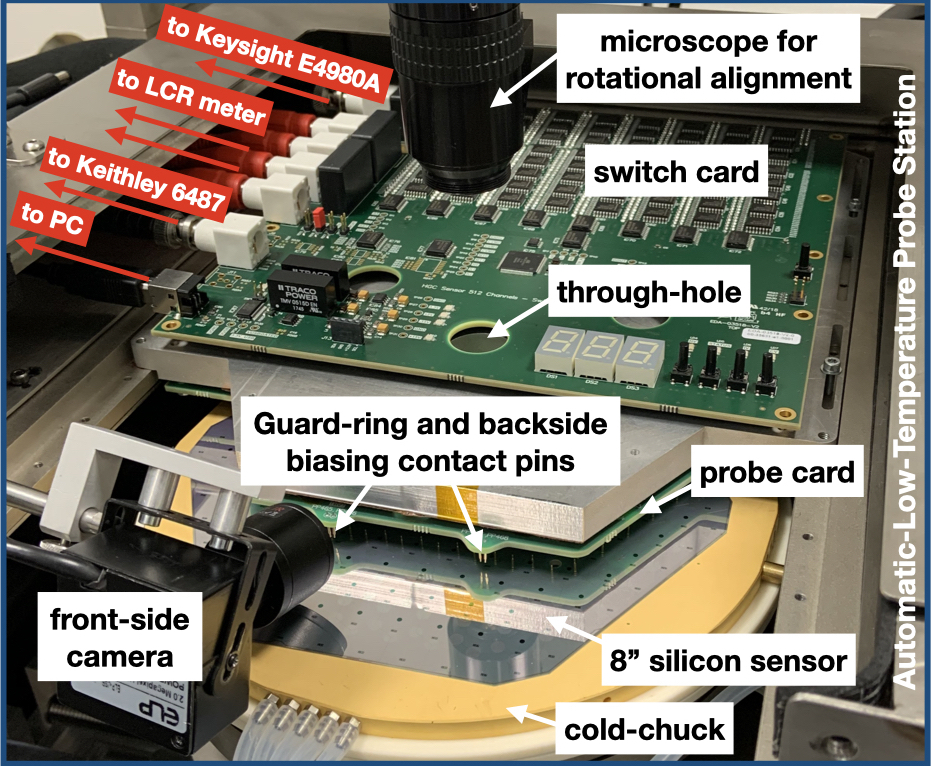
\includegraphics[width=0.75\textwidth]{figures/ALPS_photo_edit.jpeg}
	\caption{
		Silicon sensor right before connecting to the switch- and probe-card ARRAY system inside the Automatic-Low-Temperature-Probe Station (ALPS) at CERN for the testing of neutron-irradiated CMS HGCAL silicon sensor prototypes.
		The probe station was closed and flushed with dry air during the testing to prevent the formation of ice.
		}
		\label{fig:ALPS_setup}
	\end{figure}
The silicon wafers were first placed on the chuck and then connected to the probe- and switch-card based ARRAY system~\cite{pitters:array2019}.
Through-holes in the cards and the probe station's microscope  enable sufficient sensor-to-pin alignment. 
The high voltage from the Keithley 2410 power supply was provided to the chuck and to the sensor's backside.
Two probe cards specific for the high- and for the low-density sensor layouts had been designed and manufactured for the tests.
Exploiting the availability of a dedicated pad, also the guard ring could be connected through pins on the probe cards.
The switch card was operated with a bias resistance (R$_\text{bias}$) of \SI{1}{\mega\ohm} and a high voltage resistance (R$_\text{HV}$) of \SI{12}{\kilo\ohm}.
In this configuration, the ARRAY system is designed to withstand total leakage currents up to $\mathcal{O}(\SI{1}{\milli\ampere})$ and per-pad currents up to \SI{10}{\micro\ampere}.
Cooling the neutron-irradiated sensors down to \SI{-40}{\celsius} was therefore imperative.
The spatial variation of the chuck's temperature profile at this temperature amounts to $\pm\SI{0.5}{\celsius}$, cf.~\ref{appendix:chuck_temp}, whereas fluctuations with time are found to be negligible. 
In order to prevent the formation of ice, the probe station had to be flushed with dry air. 
With total currents at the order of $\mathcal{O}(\SI{1}{\milli\ampere})$, the voltage drop at R$_\text{HV}$ for the testing of neutron-irradiated sensors is non-negligible and is corrected for in \ref{sec:results}.
The voltage at the silicon pad under test is referred to as "effective bias voltage" in this work.
Per-pad leakage currents were measured with a Keithley 6487 picoammeter, whereas total currents were measured directly with the Keithley 2410 power supply.
A Keysight E4980A LCR meter was operated at a frequency (f$_\text{LCR}$) of \SI{2}{\kilo\hertz} for the inference of the per-pad impedance.
This particular frequency was chosen to minimise the error associated to the capacitance~\cite{pitters:array2019}.
It was found empirically that the impact on the end capacitance is negligible whereas the derived depletion voltages are increased by about \SI{10}{\percent} when reducing f$_\text{LCR}$ to \SI{500}{\hertz}. 

\subsection{Measurement Procedure}
\label{subsec:setup_procedure}
After connecting the sensor to the probecard, per-pad leakage currents as a function of the bias voltage (IV) for the full sensor were measured first, preceded by a per-pad capacitance vs. bias voltage assessment (CV).
After each iteration over all pads a given bias voltage, voltages were incremented up to \SI{850}{\volt}, whereby the exact choice depended on the measurement type and on the sensor thickness, or up to a maximum total leakage current of \SI{2}{\milli\ampere}.  
Pads whose leakage currents exceeded \SI{5}{\micro\ampere} were not measured any further and in particular were excluded from the subsequent CV.
The entire characterisation sequence is fully automatised as a LabView-based program (HexDAQ version 1.5.1~\cite{labview_hexdaq}).
Including voltage ramps and settling times, IV measurements of low-density sensors took about \SI{1.5}{\hour} (CV: \SI{2.5}{\hour}), whereby the duration was about twice as long for high-density sensors.
IV and CV measurements were performed both before and after a beneficial annealing for \SI{80}{\min} at \SI{60}{\celsius}\footnote{Corresponding to about two weeks at room temperature.}